%
% problemstellung.tex -- Beispiel-File für die Beschreibung des Problems
%
% (c) 2020 Prof Dr Andreas Müller, Hochschule Rapperswil
%
\section{Iteration der logistischen Gleichung
\label{logistic:section:analyse}}
\rhead{Iteration der logistischen Gleichung}

Im Abschnitt \ref{buch:section:iteration} haben wir uns
bereits mit dem Iterieren von Funktionen befasst. 
Genau dieses Prinzip der Iteration finden wir auch bei
der logistischen Gleichung wieder. 
Jede Berechnung der Population im Folgejahr ist 
eine Iteration der logistische Gleichung.
Die logistische Gleichung \eqref{eq:logistic} könnte man 
auch als Funktion $f(x) = \lambda x(1-x)$ schreiben.
Jede Iteration ist nun eine Verschachtelung von $f(x)$,
somit lässt sich jeder beliebige Wert $x_n$ auch wie folgt berechnen:  
\begin{itemize}
    \item $x_1 = f(x_0)$
    \item $x_2 = f(x_1) = f(f(x_0))$
    \item $x_3 = f(x_2) = f(f(f(x_0)))$
    \item $x_4 = f(x_3) = f(f(f(f(x_0))))$
    \item $x_5 = ...$
\end{itemize}

Wir haben im Kapitel 
\ref{logistic:section:einleitung} 
bereits beobachtet,
dass die logistische Gleichung beim Iterieren für 
verschiedene Werte von $\lambda$ gegen verschiedene 
Endwerte konvergiert. 
Der Anfangswert $x_0$ scheint dabei keine Rolle zu spielen
solange er sich im Bereich $0 < x < 1$ befindet, 
er beinflusst lediglich die Form der Kurve, 
bevor sie den Konvergenzwert erreicht. 
Das heisst, wir können $x_0$ einfach auf einen bestimmten Wert, 
zum Beispiel 0.1, setzen. 
Nun können wir $\lambda$ ebenfalls auf einen bestimmten Wert setzen
und die logistische Gleichung endlos iterieren, 
um zu sehen, gegen welchen Wert $x_n$ schliesslich konvergiert.
Mit dem Computer können natürlich nicht unendlich viele Iterationen
durchgeführt werden, aber wenn $n$ gross genug ist, 
kommt man doch sehr nahe an den tatsächlichen Konvergenzwert. 
Genau dieser Prozess ist nun in Abbildung \ref{fig:map_1} 
ersichtlich. 
Sie zeigt einen Plot, 
auf dem die horizontale Achse die verschiedenen Werte
von $\lambda$ im Bereich für $0 \leq \lambda \leq 4$ annimmt 
und die vertikale Achse anzeigt,
auf welchem Wert $x_n$ konvergiert, wenn $n$ gegen
unendlich läuft. Dabei werden einige Eigenschafen 
von der Iteration der logistischen Gleichung ersichtlich:
\begin{figure}
    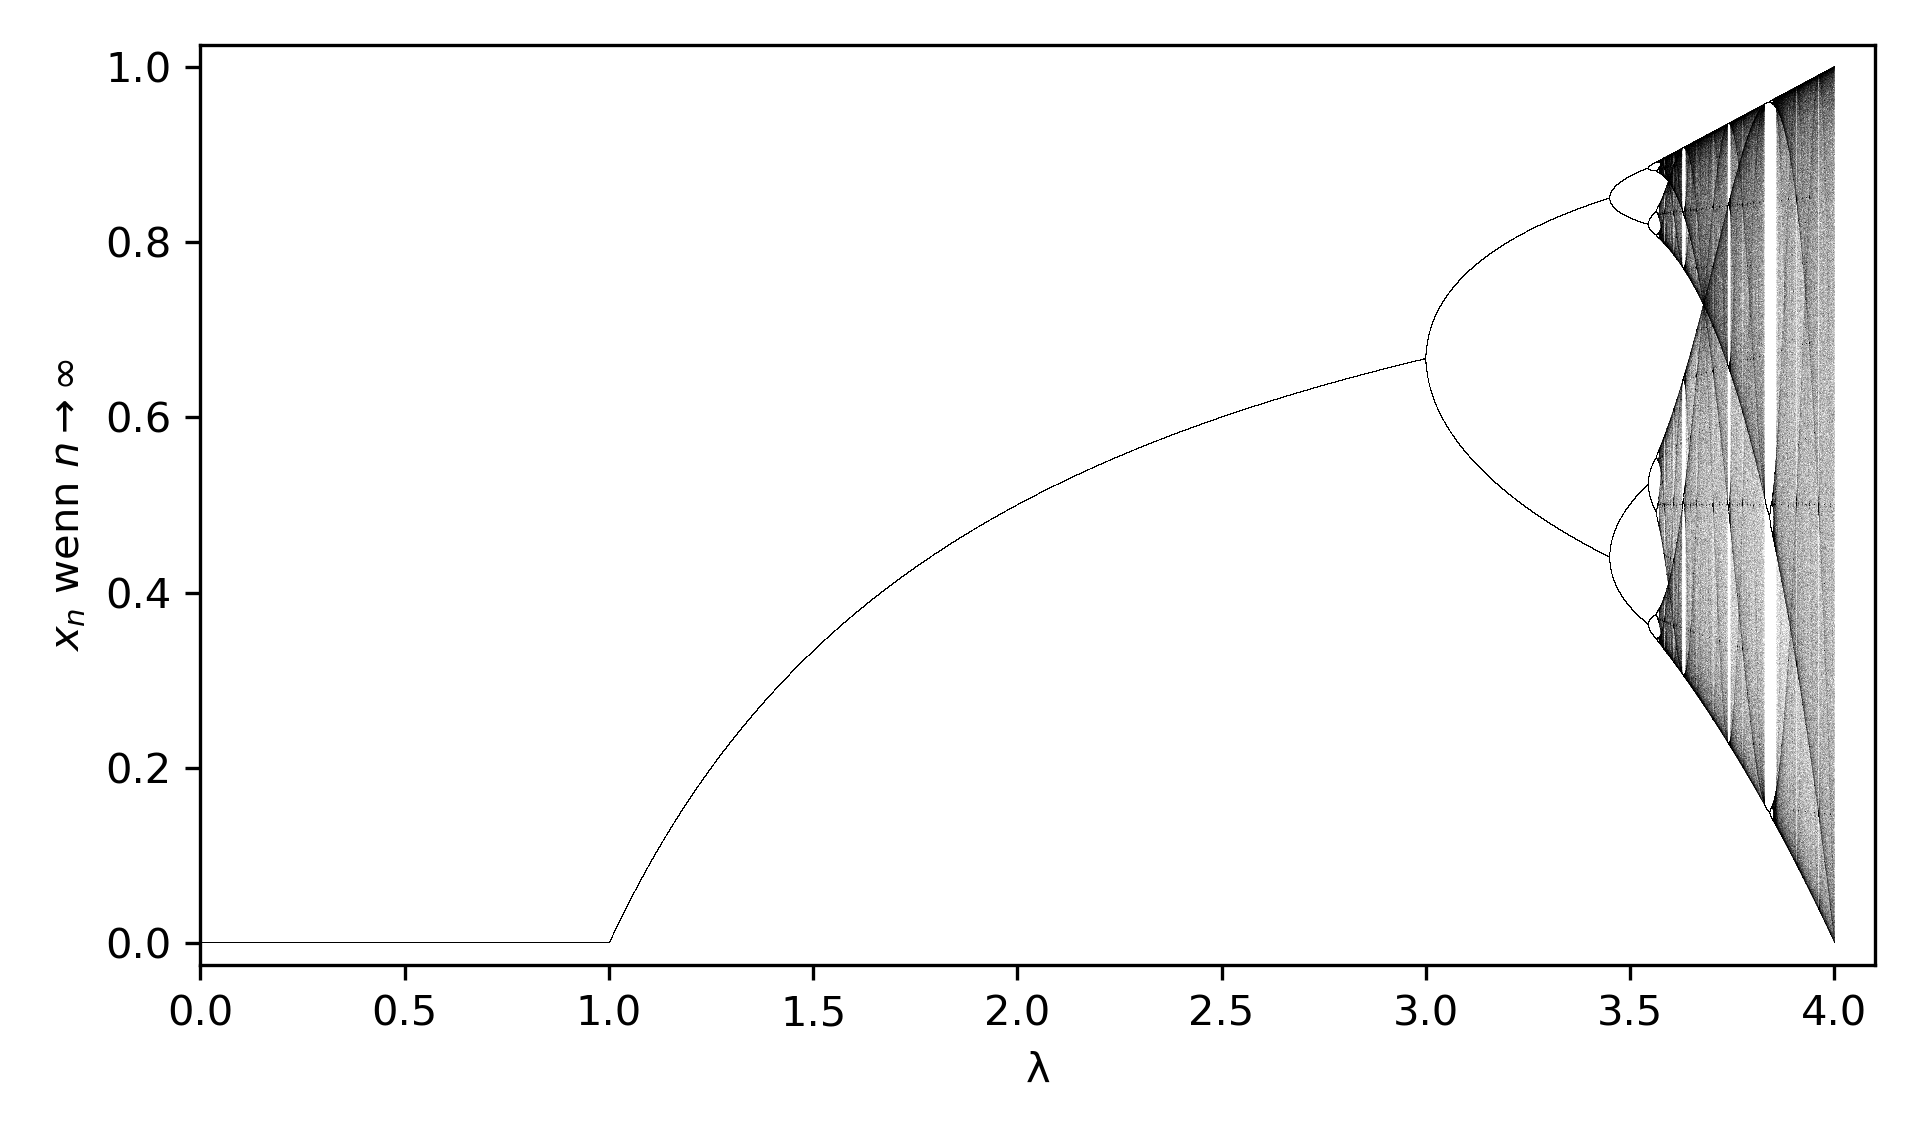
\includegraphics[width=\linewidth]{papers/logistic/figures/map.png}
    \caption{
        Bifurkationsdiagramm der logistischen Gleichung \eqref{eq:logistic}.
        Das Diagramm zeigt für jeden Wert von $\lambda$
        welche Werte $x_n$ annimmt wenn $n \rightarrow \infty$.
    }
    \label{fig:map_1}
\end{figure}
\begin{itemize}
    \item 
    für $0 \le \lambda \le 1$ konvergiert $x_n$ gegen 0
    \item 
    für $1 \le \lambda \le 3$ konvergiert $x_n$ gegen einen fixen Wert
    \item 
    für $3 \le \lambda \le 4$ scheint $x_n$ nicht mehr gegen einen fixen Wert zu konvergieren.
    Stattdessen gibt es diese Verzweigungen, 
\index{Verzweigung}%
    die darauf hindeuten, 
    dass $x_n$ zuerst bis $\lambda \approx 3.4$ zwischen zwei Werten hin und her oszilliert, 
    dann bis $\lambda \approx 3.6$ zwischen vier Werten, dann 8, 16, usw. 
    Dieses Phänomen wird auch ``Periodenverdoppelung'' genannt.
\index{Periodenverdoppelung}%
    \item
    für $\lambda > 4$ gibt es scheinbar nichts mehr.
    Das kommt daher, dass $x_n$ ab da nur noch divergiert.  
\end{itemize}
\begin{figure}
    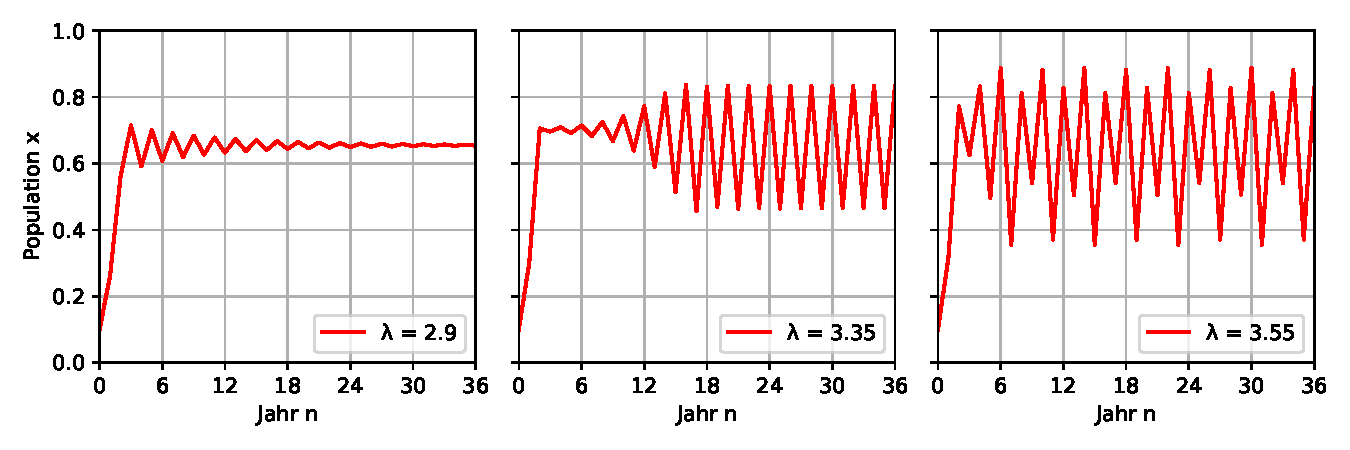
\includegraphics[width=\linewidth]{papers/logistic/figures/pop_logistic_2.pdf}
    \caption{
        Iteration der logistischen Gleichung. 
        Für $\lambda = 2.9$ konvergiert $x_n$ gegen
        $\approx 0.62$.
        Im Kontrast dazu oszilliert $x_n$ für
        $\lambda = 3.35$ und zwischen zwei 
        und für
        $\lambda = 3.55$ sogar zwischen vier Werten. 
    }
    \label{fig:pop_logistic_2}
\end{figure}
Das doch eher spezielle Verhalten von $3 < \lambda < 4$ wird 
auch in Abbildung \ref{fig:pop_logistic_2} ersichtlich,
wenn man die Werte der einzelnen Iteration plottet.
Im ersten Plot mit $\lambda = 2.9$ sieht man, dass $x_n$ zuerst oszilliert,
aber schliesslich auf einen fixen Wert konvergiert.
Auf dem zweiten Plot mit $\lambda = 3.35$ scheint $x_n$ 
nach einigen Iterationen nur noch
zwischen zwei Werten zu oszillieren und beim
dritten Plot mit $\lambda = 3.55$ sogar zwischen vier Werten. 
Dieses Oszillieren zeigt sich in Abbildung \ref{fig:map_1}
durch die Verzweigungen oder auch ``Bifurkationen''. 
\index{Bifurkation}%
\index{Bifurkationsdiagramm}%
Darum wird sie auch ``Bifurkationsdiagramm'' genannt. 

Auf dem Bifurkationsdiagramm sind noch mehr 
interessante Eigenschaften der logistischen Gleichung erkennbar.
Wenn wir, wie in Abbildung \ref{fig:map_zoom}, in die Bereiche hineinzoomen
wo die Bifurkationen immer dichter werden, finden wir Gebilde, 
welche wieder fast genau gleich aussehen.
Tatsächlich könnte man endlos immer weiter in diese
Bereiche hineinzoomen und würde immer wieder auf solche änhlichen Muster stossen. 
Diese Selbstähnlichkeit ist eine typische Eigenschaft von Fraktalen.
\index{Selbstähnlichkeit}%
\index{Fraktal}%
Das Bifurkationsdiagramm der logistischen Gleichung ist also ein Fraktal.
Es gibt sogar einen Zusammenhang zwischen der logistischen Gleichung und 
einem anderen berühmten Fraktal, der Mandelbrotmenge.
\index{Mandelbrotmenge}%
Mehr dazu später in Abschnitt 
\ref{logistic:section:beispiele}.
\begin{figure}
    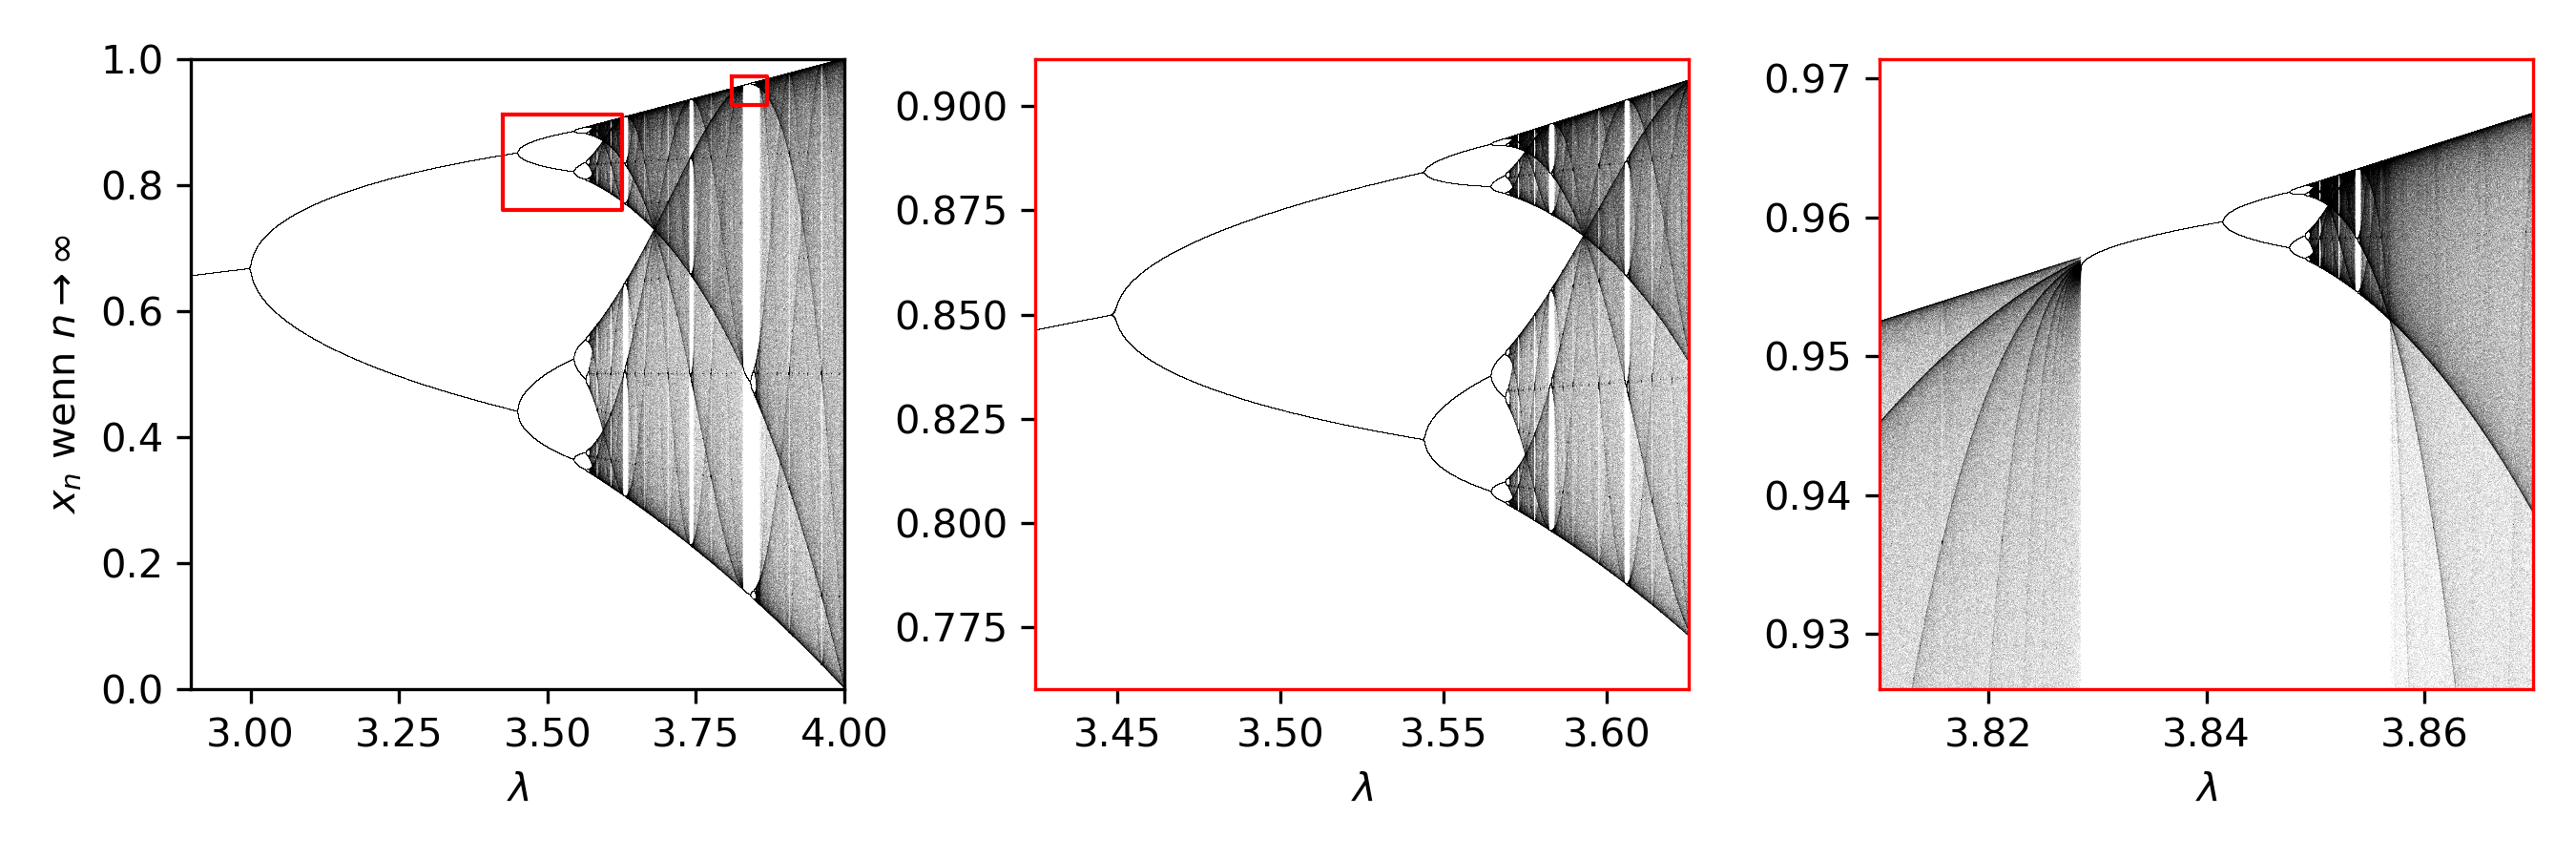
\includegraphics[width=\linewidth]{papers/logistic/figures/map_zoom.png}
    \caption{
        Das Bifurkationsdiagramm ist ein Fraktal.
        Die mittlere Grafik verdeutlicht mit einem Zoom 
        bei $\lambda = 3.525$ die Selbstänhlichkeit. 
        Auf der rechten Grafik sieht man mit einem
        Zoom bei $\lambda = 3.84$, dass sich immer
        wieder das selbe Muster finden lässt.
    }
    \label{fig:map_zoom}
\end{figure}

Des weiteren ist auf dem Bifurkationsdiagramm zu sehen,
dass für jede weitere Periodenverdoppelung eine geringere
Erhöhung von $\lambda$ notwendig ist.
Diese rapide zunehmende Dichte der Periodenverdoppelungen führt dazu, 
dass wenn $\lambda$ den Wert $\approx 3.57$ überschreitet, 
die Verdoppelungen aufhören und $x_n$ nicht mehr oszilliert. 
Stattdessen nimmt $x_n$ nur noch scheinbar 
willkürliche Werte in bestimmten Bereichen an, 
man spricht vom Chaos.
\index{Chaos}
Interessanterweise gibt es aber auch für Werte von 
$\lambda \gtrapprox 3.57$ wieder gewissen Bereiche,
wo wieder periodisches Verhalten auftritt. 
Ein Beispiel für einen solchen Bereich sieht man
gut in Abbildung \ref{fig:map_zoom} bei 
$\lambda \approx 3.83$. 
Dort gibt es zuerst eine Dreier-Periode, 
dann wieder die Periodenverdoppelungen, 
wobei die Dichte der Verdoppelungen
wieder rapide zunimmt.
Schliesslich bricht wieder das Chaos aus bei 
$\lambda \approx 3.85$.
